\documentclass[authoryearcitations]{UoYCSproject}

\usepackage{tikz}
\usetikzlibrary{arrows,positioning}

\tikzset{
    vertex/.style={circle,draw,minimum size=10mm},
    invisible/.style={minimum size=10mm},
    pre/.style={->,semithick},
    post/.style={<-,semithick}
}

\usepackage{mathtools}
\usepackage{amsmath}

\author{Joshua Asch}

\title{Tracing and Debugging in GP2}

\date{Date TBC}
\supervisor{Detlef Plump}
\MEng
\wordcount{3577}


\abstract{
The University of York has developed a graph programming language, GP2 (Graph
Programs 2), which has a small IDE. In this project, new features are designed,
implemented, and evaluated which allow users to step through a GP2 program in
the IDE.
}


\begin{document}

\maketitle
\listoffigures
\listoftables

\cleardoublepage

%XXXXXXXXXXXXXXXXXXXXXXXXXXXXXXXXXXXXXXXXXXXXXXXXXXXXXXXXXXXXXXXXXXXXXXXXXXXXXX

\chapter{Introduction}
\label{cha:Introduction}

\section{Motivation}
\label{sec:Motivation}

\emph{Introduce the project, explain why the project needs doing}

%==============================================================================

\section{Ethics}
\label{sec:Ethics}

\emph{Discuss the ethical considerations for the project, which there may
not be any at all, if no humans are involved.}

\clearpage

%XXXXXXXXXXXXXXXXXXXXXXXXXXXXXXXXXXXXXXXXXXXXXXXXXXXXXXXXXXXXXXXXXXXXXXXXXXXXXX

\chapter{Literature Review}
\label{cha:LiteratureReview}

\section{Programming by Graph Transformation}
\label{sec:ProgrammingByGraphTransformation}

\subsection{Graph Programming}
\label{sec:GraphProgramming}

Graph programming involves a series of transformations applied to a graph. The
problem being solved must be redefined in terms of a start graph and an algorithm
represented by graph transformations. The final graph at the end of the algorithm
gives the solution to the problem.

Historically, programming by graph transformation required using a programming
language such as C or Java, implementing data structures to represent graphs, and
directly making modifications to the graph in the program. However, recently some
attempts have been made to create tools for graph programming which abstract away
the representation of the graphs, allowing the programmer to focus on the program itself.

Some of these tools include GROOVE \citep{GROOVE2012}, AGG \citep{ermel1999},
GrGen \citep{GrGen2010}, and, most recently, GP2 \citep{plump2012}. All of these
are domain-specific languages for graph programming which also provide a graphical
interface to describe graphs and transformations.

These kinds of tools take a representation of a graph program, as defined in their
graphical editor, and transform this into a runnable program. This can be implemented
in a number of languages, including Java (in the case of AGG and GROOVE), C\# .NET
(GrGen), or C (GP2). This program can then be executed to find the output graph
generated by the algorithm.

%==============================================================================

\subsection{The GP2 Language}
\label{sec:TheGP2Language}

GP2 (Graph Programs 2) is a programming language developed at the University of
York \citep{plump2012,bak2015}, an updated implementation of the original language,
GP \citep{plump2009}. It is designed for writing programs at a high level, to
perform graph transformations without having to implement data structures to
represent the graphs in more traditional lower level languages such as C.

Programming in GP2 consists of an input graph, known as the \emph{host graph}, a
set of \emph{rules}, and a \emph{program} which defines the order in which to
apply the rules. Running a GP2 program on a host graph produces a new graph as
a result, called the \emph{output graph}.

%------------------------------------------------------------------------------

\subsubsection{Rules}
\label{sec:Rules}

\begin{figure}
    \begin{center}
        \begin{tabular}{l}

            \texttt{link}

            \\

            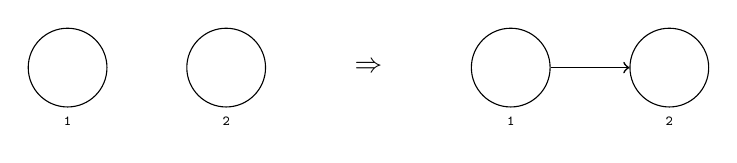
\begin{tikzpicture}

                \node         (transition) {$\Rightarrow$}            {};

                \node[vertex] (lhs 2) [label=below:\tiny{\texttt{2}},left=of transition]  {};
                \node[vertex] (lhs 1) [label=below:\tiny{\texttt{1}},left=of lhs 2]       {};

                \node[vertex] (rhs 1) [label=below:\tiny{\texttt{1}},right=of transition] {};
                \node[vertex] (rhs 2) [label=below:\tiny{\texttt{2}},right=of rhs 1]      {}
                    edge[post] (rhs 1);

            \end{tikzpicture}

            \\

            \texttt{where not edge(1, 2)}

        \end{tabular}
    \end{center}
    \caption{A rule in GP2}
    \label{fig:RuleInGP2}
\end{figure}

Rules are the basic building blocks of a GP2 program and are defined by a
left-hand-side (LHS), a right-hand-side (RHS), and optionally a conditional
clause. A rule can be thought of as the definition of a transformation; a subgraph
matching the LHS of the rule is transformed to resemble the RHS. An example of a
GP2 rule is shown in \autoref{fig:RuleInGP2}.

The conditional clause is used to specify additional constraints on the subgraph
matching the LHS. Any match has to both match the LHS and conform to the constraints
defined by the conditional clause.

In a compiled program, a rule is split into two phases. The \emph{match} phase
searches the current graph for a subgraph which matches the LHS of the rule. This must
be an \emph{injective match}, meaning that each item in the LHS must be matched with
exactly one item in the host graph.

In this implementation of GP2, rule matches are chosen determinstically due to the
impracticality of generating all non-deterministic possibilities, which is what GP1 did.
If no match is found for the LHS, the rule is considered \emph{failed}. If a match is
found, the program moves on to the second phase, the \emph{application}.

A rule specifies a number of \emph{interface nodes}, nodes which are present in both
the LHS and the RHS. These interface nodes can be seen in \autoref{fig:RuleInGP2}; they
are the nodes with small numeric labels. During the application phase, any nodes in the
LHS which are \emph{not} interface nodes will be deleted. Similarly, any non-interface
nodes which appear in the RHS will be created. At the end of the application phase,
the subgraph will match the RHS of the rule definition. The new graph created by the
application of this rule, an \emph{intermediate graph}, is then used as the input to
the next part of the program.

In the example in \autoref{fig:RuleInGP2}, the program will search for a subgraph
containing two nodes without an edge connecting them. If a match is found, it will
be transformed to resemble the RHS by adding an edge between the nodes.

%------------------------------------------------------------------------------

\subsubsection{The Dangling Condition}
\label{sec:TheDanglingCondition}

\begin{figure}
    \begin{center}
        \begin{tabular}{l}

            \texttt{delete}

            \\

            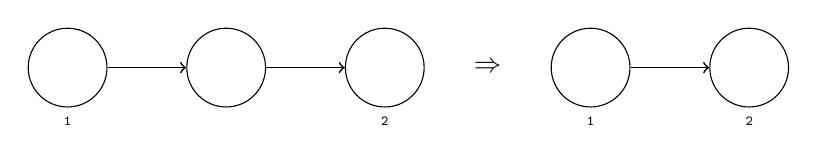
\begin{tikzpicture}

                \node         (transition) {$\Rightarrow$}            {};

                \node[vertex] (lhs 3) [label=below:\tiny{\texttt{2}},left=5mm of transition]  {};
                \node[vertex] (lhs 2) [left=of lhs 3]                                     {}
                    edge[pre] (lhs 3);
                \node[vertex] (lhs 1) [label=below:\tiny{\texttt{1}},left=of lhs 2]       {}
                    edge[pre] (lhs 2);

                \node[vertex] (rhs 1) [label=below:\tiny{\texttt{1}},right=5mm of transition] {};
                \node[vertex] (rhs 2) [label=below:\tiny{\texttt{2}},right=of rhs 1]      {}
                    edge[post] (rhs 1);

            \end{tikzpicture}

            \\\\\\

            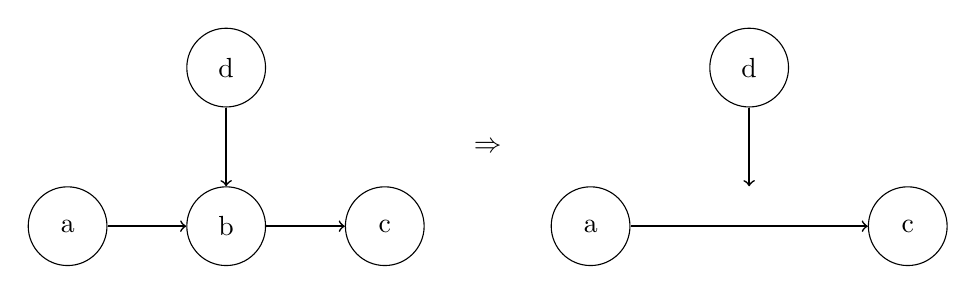
\begin{tikzpicture}

                \node (transition) {$\Rightarrow$} {};

                \node[vertex] (lhs c) [left=5mm of transition, yshift=-10mm] {c} {};
                \node[vertex] (lhs b) [left=of lhs c]                    {b} {}
                    edge[pre] (lhs c);
                \node[vertex] (lhs a) [left=of lhs b]                    {a} {}
                    edge[pre] (lhs b);
                \node[vertex] (lhs d) [above=of lhs b]                   {d} {}
                    edge[pre] (lhs b);


                \node[vertex]     (rhs a)         [right=5mm of transition, yshift=-10mm] {a} {};
                \node[invisible]  (rhs invisible) [right=of rhs a]                            {};
                \node[vertex]     (rhs c)         [right=of rhs invisible]                {c} {}
                    edge[post]    (rhs a);
                \node[vertex]     (rhs d)         [above=of rhs invisible]                {d} {}
                    edge[pre]     (rhs invisible);

            \end{tikzpicture}

        \end{tabular}
    \end{center}
    \caption{Attempting to apply a rule when the match violates the dangling condition}
    \label{fig:FailDanglingCondition}
\end{figure}

There is an additional condition which determines whether a rule can be matched, the
\emph{dangling condition}. This condition states that if a rule causes a node to be
deleted, the rule must also delete all edges incident to that node. In
other words, all non-interface nodes in a rule match must have no incoming or outgoing
edges which are not also part of the match.

\autoref{fig:FailDanglingCondition} shows the result of attempting to apply a rule
where the match violates the dangling condition. Since node b is not an interface
node, it is deleted during the application of the \texttt{delete} rule. However, the
rule does not specify that the edge from b to d should be deleted. This leaves a
\emph{dangling edge} from node d with no target. The dangling condition is used to
ensure that rules result in no dangling edges.

%------------------------------------------------------------------------------

\subsubsection{Programs}
\label{sec:Programs}

A GP2 program defines the order in which to apply rules using 8 simple control
structures:

\begin{description}
    \item[\textsc{Sequence}]
    Two subprograms separated by a semicolon ``\texttt{P; Q}'' are applied
    one after the other.

    \item[\textsc{Rule Set}]
    Rules in curly braces ``\texttt{\{R$_{\text{1}}$, R$_{\text{2}}$, R$_{\text{3}}$\}}''
    define a set, where exactly one rule from the set is executed, unless no rule in
    the set can be matched. The implementation of GP2 selects a rule determinstically,
    though the the specification allows non-determinism.

    \item[\textsc{If-Then-Else}]
    In the statement ``\texttt{if C then P else Q}'', the sub-program \texttt{C}
    is executed, and the result, i.e. success or failure, is recorded, before
    reverting any changes caused by C. Then, if C succeeded, \texttt{P} is
    executed on the original graph. If it failed, then \texttt{Q} is executed on
    the original graph. Note that by taking a copy first, any changes made by
    \texttt{C} are reverted before executing either \texttt{P} or \texttt{Q}.

    \item[\textsc{Try-Then-Else}]
    Similar to \textsc{If-Then-Else}, but \texttt{C} is only reverted if it fails.
    Thus any changes made by \texttt{C} are \emph{not} reverted before executing
    \texttt{P}, but they \emph{are} reverted before executing \texttt{Q}.

    \item[\textsc{As-Long-As-Possible}]
    A subprogram followed by an exclamation point ``\texttt{P!}'' is matched and
    applied repeatedly until it fails. When \texttt{P} fails, it does not transition
    the program to the fail state.

    \item[\textsc{Procedure}]
    Similar to a C preprocessor macro, a procedure is simply a named subprogram
    where any reference to the procedure name can be replaced with the definition
    of the procedure.

    \item[\textsc{Skip}]
    A no-op which always succeeds, and does not affect the graph. Invoked using the
    keyword ``\texttt{skip}''.

    \item[\textsc{Fail}]
    A no-op which always fails and does not affect the graph. This is the same as
    attempting to execute a rule for which there are no matches. Invoked using
    the keyword ``\texttt{fail}''.
\end{description}

For GP2, a subprogram is either a single rule, referenced by its name, or one of
the above control structures. Therefore it is possible to nest control structures
to create more complex programs.

In general, execution of a program continues until either all statements are
executed, or until a statement results in an attempt to apply a rule which has
no matches in the graph. The exceptions to this are \textsc{As-Long-As-Possible}
statements, and the conditional statements in \textsc{If-Then-Else} and
\textsc{Try-Then-Else} structures. In these cases, a failure to match a rule
does not halt execution of the program.

\autoref{fig:ExampleProgramDefinition} shows an example GP2 program, an adapted
version of the program used as a case study in Bak's thesis on GP2 \citep[p.126]{bak2015}.
It is a simple program which determines whether a graph is \emph{2-colourable},
that is, its nodes can be coloured using two different colours without two nodes
of the same colour being connected by an edge.

This program consists of four rules and uses many of the constructs outlined
previously, including \textsc{Try-Then-Else}, \textsc{If-Then-Else},
\textsc{Rule Set}s, \textsc{As-Long-As-Possible} and \textsc{Procedure}s.

It also takes advantage of another feature of GP2, the ability to \emph{colour}
a node. The colour of a node is a property which can be set by a rule, or the
host graph can contain coloured nodes. The colour is taken into account when
searching for a rule match; for example, in this program, \texttt{joined\_reds}
will only match when both the nodes' colours are red.

\begin{figure}
    \begin{center}
        \begin{verbatim}
Main = try (init; Colour!; if Invalid then fail)
Colour = {colour_blue, colour_red}
Invalid = {joined_reds, joined_blues}
        \end{verbatim}

        \begin{tabular}{l}            

            \texttt{init}

            \\ 

            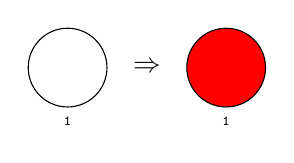
\begin{tikzpicture}

                \node         (transition) {$\Rightarrow$}                                       {};

                \node[vertex] (lhs) [label=below:\tiny{\texttt{1}},left=2mm of transition]           {};

                \node[vertex] (rhs) [label=below:\tiny{\texttt{1}},right=2mm of transition,fill=red] {};

            \end{tikzpicture}

            \\\\

            \texttt{joined\_reds}

            \\

            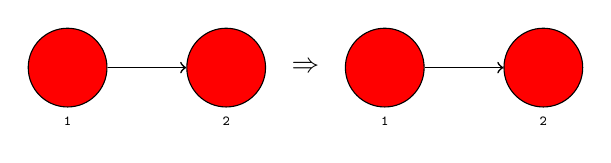
\begin{tikzpicture}

                \node         (transition) {$\Rightarrow$}                                         {};

                \node[vertex] (lhs 2) [label=below:\tiny{\texttt{2}},left=2mm of transition,fill=red]  {};
                \node[vertex] (lhs 1) [label=below:\tiny{\texttt{1}},left=of lhs 2,fill=red]       {}
                    edge[pre] (lhs 2);

                \node[vertex] (rhs 1) [label=below:\tiny{\texttt{1}},right=2mm of transition,fill=red] {};
                \node[vertex] (rhs 2) [label=below:\tiny{\texttt{2}},right=of rhs 1,fill=red]      {}
                    edge[post] (rhs 1);

            \end{tikzpicture}

            \\\\

            \texttt{joined\_blues}

            \\

            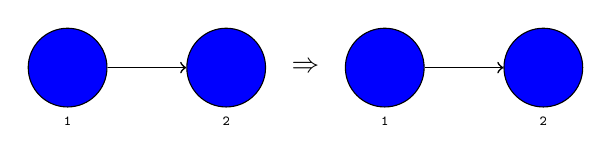
\begin{tikzpicture}

                \node         (transition) {$\Rightarrow$}                                          {};

                \node[vertex] (lhs 2) [label=below:\tiny{\texttt{2}},left=2mm of transition,fill=blue]  {};
                \node[vertex] (lhs 1) [label=below:\tiny{\texttt{1}},left=of lhs 2,fill=blue]       {}
                    edge[pre] (lhs 2);

                \node[vertex] (rhs 1) [label=below:\tiny{\texttt{1}},right=2mm of transition,fill=blue] {};
                \node[vertex] (rhs 2) [label=below:\tiny{\texttt{2}},right=of rhs 1,fill=blue]      {}
                    edge[post] (rhs 1);

            \end{tikzpicture}

            \\\\

            \texttt{colour\_red}

            \\

            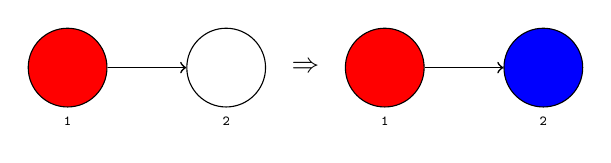
\begin{tikzpicture}

                \node         (transition) {$\Rightarrow$}                                          {};

                \node[vertex] (lhs 2) [label=below:\tiny{\texttt{2}},left=2mm of transition]            {};
                \node[vertex] (lhs 1) [label=below:\tiny{\texttt{1}},left=of lhs 2,fill=red]        {}
                    edge[pre] (lhs 2);

                \node[vertex] (rhs 1) [label=below:\tiny{\texttt{1}},right=2mm of transition,fill=red]  {};
                \node[vertex] (rhs 2) [label=below:\tiny{\texttt{2}},right=of rhs 1,fill=blue]      {}
                    edge[post] (rhs 1);

            \end{tikzpicture}

            \\\\

            \texttt{colour\_blue}

            \\

            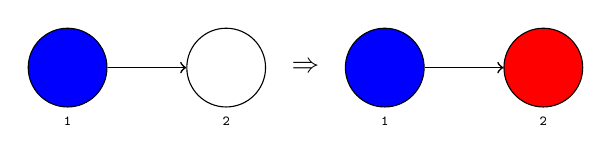
\begin{tikzpicture}

                \node         (transition) {$\Rightarrow$}                                          {};

                \node[vertex] (lhs 2) [label=below:\tiny{\texttt{2}},left=2mm of transition]            {};
                \node[vertex] (lhs 1) [label=below:\tiny{\texttt{1}},left=of lhs 2,fill=blue]       {}
                    edge[pre] (lhs 2);

                \node[vertex] (rhs 1) [label=below:\tiny{\texttt{1}},right=2mm of transition,fill=blue] {};
                \node[vertex] (rhs 2) [label=below:\tiny{\texttt{2}},right=of rhs 1,fill=red]       {}
                    edge[post] (rhs 1);

            \end{tikzpicture}

        \end{tabular}
    \end{center}
    \caption{Definition of 2-colouring in GP2}
    \label{fig:ExampleProgramDefinition}
\end{figure}

\begin{figure}
    \begin{center}
        \begin{tabular}{l}    

            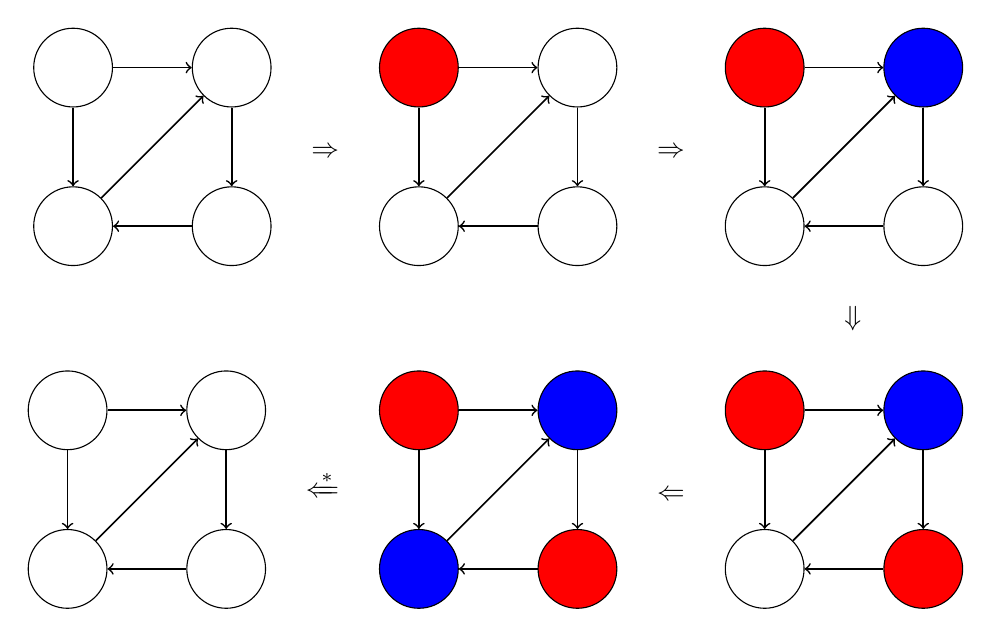
\begin{tikzpicture}
                [vertex/.style={circle,draw,minimum size=10mm}]

                \node (transition1) {$\Rightarrow$} {};

                \node[vertex]  (12) [above left=7.5mm of transition1] {};
                \node[vertex]  (13) [below=of 12]               {}
                    edge[post] (12);
                \node[vertex]  (11) [left=of 12]                {}
                    edge[pre]  (12);
                \node[vertex]  (14) [below=of 11]               {}
                    edge[post] (11)
                    edge[pre]  (12)
                    edge[post] (13);

                \node[vertex]  (21) [above right=7.5mm of transition1,fill=red] {};
                \node[vertex]  (22) [right=of 21]                         {}
                    edge[post] (21);
                \node[vertex]  (23) [below=of 22]                         {}
                    edge[post] (22);
                \node[vertex]  (24) [below=of 21]                         {}
                    edge[post] (21)
                    edge[pre]  (22)
                    edge[post] (23);

                \node (transition2) [below right=7.5mm of 22] {$\Rightarrow$} {};

                \node[vertex]  (31) [above right=7.5mm of transition2,fill=red] {};
                \node[vertex]  (32) [right=of 31,fill=blue]               {}
                    edge[post] (31);
                \node[vertex]  (33) [below=of 32]                         {}
                    edge[post] (32);
                \node[vertex]  (34) [below=of 31]                         {}
                    edge[post] (31)
                    edge[pre]  (32)
                    edge[post] (33);

                \node (transition3) [below right=7.5mm of 34] {$\Downarrow$} {};

                \node[vertex]  (41) [below left=7.5mm of transition3,fill=red] {};
                \node[vertex]  (42) [right=of 41,fill=blue]                  {}
                    edge[post] (41);
                \node[vertex]  (43) [below=of 42,fill=red]                   {}
                    edge[post] (42);
                \node[vertex]  (44) [below=of 41]                            {}
                    edge[post] (41)
                    edge[pre]  (42)
                    edge[post] (43);

                \node (transition4) [below left=7.5mm of 41] {$\Leftarrow$} {};

                \node[vertex]  (52) [above left=7.5mm of transition4,fill=blue] {};
                \node[vertex]  (51) [left=of 52,fill=red]                   {}
                    edge[pre]  (52);
                \node[vertex]  (53) [below=of 52,fill=red]                  {}
                    edge[post] (52);
                \node[vertex]  (54) [below=of 51,fill=blue]                  {}
                    edge[post] (51)
                    edge[pre]  (52)
                    edge[post] (53);

                \node (transition5) [below left=7.5mm of 51, yshift=2.5mm] {$\xLeftarrow{*}$} {};

                \node[vertex]  (62) [above left=7.5mm of transition5, yshift=-2.5mm] {};
                \node[vertex]  (61) [left=of 62]                    {}
                    edge[pre]  (62);
                \node[vertex]  (63) [below=of 62]                   {}
                    edge[post] (62);
                \node[vertex]  (64) [below=of 61]                   {}
                    edge[post] (61)
                    edge[pre]  (62)
                    edge[post] (63);

            \end{tikzpicture}

        \end{tabular}
    \end{center}
    \caption{Example execution of 2-colouring}
    \label{fig:ExampleProgramExecution}
\end{figure}

An example execution of the 2-colouring program is shown in \autoref{fig:ExampleProgramExecution}.
Starting with an uncoloured graph, the algorithm picks a node and colours it red
using the \texttt{init} rule. It then traverses the graph colouring nodes in
alternating colours using the \texttt{colour\_blue} and \texttt{colour\_red} rules,
by defining them as a \textsc{Rule Set} in a \textsc{Procedure} and executing
it \textsc{As-Long-As-Possible}. When no more uncoloured nodes are present in the
graph, the \texttt{Colour} procedure will be unable to match any further rules,
so it will end.

To check whether the produced colouring is valid, the entire \texttt{Main}
procedure is wrapped in a \textsc{Try-Then-Else} statement. After executing
\texttt{Colour}, the \texttt{Invalid} procedure runs. This procedure uses the
two remaining rules, \texttt{joined\_reds} and \texttt{joined\_blues}, to see if
any adjacent nodes are the same colour. If they are, one of these rules will
match, triggering the conditional statement \texttt{fail} from the
\textsc{If-Then-Else} statement. This in turn causes the outer \texttt{try} to
fail, reverting all changes made to the graph and returning the uncoloured input
graph.

However, if \texttt{Invalid} fails to match either of the rules, it must mean
that no two same-coloured nodes are connected via an edge. This means that it is
a valid colouring. The \texttt{fail} statement is not executed, meaning the
\texttt{try} succeeds. The changes to the graph are kept, and the modified graph
is returned as the result of the program.

In the example execution in \autoref{fig:ExampleProgramExecution}, the host graph
is not 2-colourable. When the rules in \texttt{Colour} can no longer be matched,
\texttt{joined\_blues} inside \texttt{Invalid} will match with the nodes in the
bottom-left and top-right of the graph. Because this rule was successfully applied
(even though it has no effect on the graph), the \textsc{If-Then-Else} causes the
program to enter the fail state. This in turn means that the \textsc{Try-Then-Else}
surrounding the program fails, and all the changes made to the input graph are
reversed. The output graph is therefore identical to the input graph.

%------------------------------------------------------------------------------

\subsubsection{Labels}
\label{sec:Labels}

Nodes and edges in a graph defined in GP2 can also have \emph{labels}. Each node
or edge can either have one label or it can be unlabelled. A graph is
\emph{partially labelled} if some of the nodes and edges have labels, and it is
\emph{totally labelled} if every node and edge has a label.

Labels can be used cosmetically, without affecting the execution of the program,
or they can be included in rules to have the program read and modify labels.

\begin{figure}
    \begin{center}
        \begin{tikzpicture}
            \node (list) {\texttt{list}} {};
            \node (ss1)  [below=1mm of list] {\rotatebox{90}{$\subseteq$}} {};
            \node (atom) [below=1mm of ss1]  {\texttt{atom}} {};
            \node (ss2)  [below left=1mm of atom] {\rotatebox{45}{$\subseteq$}} {};
            \node (ss3)  [below right=1mm of atom] {\rotatebox{135}{$\subseteq$}} {};
            \node (int)  [below left=1mm of ss2] {\texttt{int}} {};
            \node (string) [below right=1mm of ss3] {\texttt{string}} {};
            \node (ss4)  [below=1mm of string] {\rotatebox{90}{$\subseteq$}} {};
            \node (char) [below=1mm of ss4] {\texttt{char}} {};

        \end{tikzpicture}
    \end{center}
    \caption{GP2's type hierarchy for labels}
    \label{fig:TypeHierarchy}
\end{figure}

GP2 has a type hierarchy for labels, shown in \autoref{fig:TypeHierarchy}. Labels
can be of any of these five types. An \texttt{atom} consists of a single entity,
either an \texttt{int} or a \texttt{string}. A \texttt{list} is a collection of
\texttt{atom}s concatenated together; the concatenation is shown using a colon
(\texttt{:}).

When matching a rule involving labels, GP2 finds a variable assignment which
matches the values of the labels in the graph. The values in this assignment are
identical when used in the RHS of the rule. When using labels in a rule, the type
of each label must be specified so that GP2 can find an assignment for each one.

\begin{figure}
    \begin{center}
        \begin{tabular}{l}
            
            \texttt{swap(x, y: int)}

            \\

            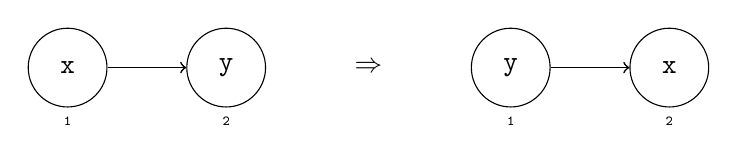
\begin{tikzpicture}

                \node         (transition) {$\Rightarrow$}            {};

                \node[vertex] (lhs 2) [label=below:\tiny{\texttt{2}},left=of transition]  {\texttt{y}}{};
                \node[vertex] (lhs 1) [label=below:\tiny{\texttt{1}},left=of lhs 2]       {\texttt{x}}{}
                    edge[pre] (lhs 2);

                \node[vertex] (rhs 1) [label=below:\tiny{\texttt{1}},right=of transition] {\texttt{y}}{};
                \node[vertex] (rhs 2) [label=below:\tiny{\texttt{2}},right=of rhs 1]      {\texttt{x}}{}
                    edge[post] (rhs 1);

            \end{tikzpicture}

            \\

            \texttt{where x > y}

        \end{tabular}
    \end{center}
    \caption{A GP2 rule which uses labels}
    \label{fig:ExampleRuleWithLabels}
\end{figure}

The rule in \autoref{fig:ExampleRuleWithLabels} will only match a pair
of nodes where the labels are both integers, and the value of the source node's
label is greater than the value of the target node's label. This rule
demonstrates both that labels can be used as conditions in the program, and also
that a rule can modify labels. It also shows that labels act like variables when
used in a rule, since the values of \texttt{x} and \texttt{y} are re-used in the
RHS.

%//////////////////////////////////////////////////////////////////////////////

\section{Tracing and Debugging}
\label{sec:TracingAndDebugging}

\subsection{Debugging in Imperative Languages}
\label{sec:DebuggingInImperativeLanguages}

When programming in a high level imperative language, such as C or Java, the
programmer will more often than not have access to a \emph{debugger}. In
\citep{sammet1969}, Sammet says that a program in a high level language without
debugger support may be ''harder to debug than an assembly language which the
programmer understands'', since the programmer has to interpret the compiled code,
rather than reading the source code they wrote.

Most language interpreters and Integrated Development Environments (IDEs) have a
debugger built in \citep{scott2009}, and standalone debuggers are also available
for some languages. For C, this may be \texttt{gdb} \citep{gdbsite}, while for
Java, it might be \texttt{jdb} \citep{jdbsite}. 

A debugger is intended to allow the programmer to pause their program during
execution, so that they can inspect the contents of variables and other memory
locations. It also allows them to run their program step-by-step to see its
execution flow; they may wish to check that a function is called at the expected
point during execution, for instance.

Some debuggers also include more advanced features to make debugging easier and to
give the programmer more insight into their program. Breakpoints are a common feature
which allow the programmer to specify a line of source code and have the program
execute normally until the breakpoint is reached, at which point execution will
pause, or \emph{break}.

Because GP2 has a rule-based structure, unlike imperative programming languages,
it is not clear what a ''line of code'' represents in a GP2 program. The textual
part of a GP2 program can indeed have lines, but since a single line in a GP2
program can be complex and use many rules, this is too high-level to consider a
''line of code'' as a debugger does. In an imperative language, a single line of
code may only perform one or two actions, so inspecting each line individually
shows the flow of the program. In GP2, running a line of the textual program
could result in tens or hundreds of rules being applied if \textsc{As-Long-As-Possible}
is used, for example. It may be inappropriate to focus on how debuggers are
implemented for imperative languages when considering GP2.

%------------------------------------------------------------------------------

\subsubsection{IDEs}
\label{sec:IDEs}

A debugger is often available from within the Integrated Development Environment
(IDE) for a language. For example, the Visual Studio IDE for C, C++, and C\#
includes the Visual Studio Debugger \citep{msdnsite}. One of the most prevalent
Java IDEs, Eclipse, integrates with \texttt{jdb} \citep{eclipsesite}.

When an IDE integrates with a debugger, it can provide additional functionality
by allowing the programmer to interact with the source code and the debugger
visually in the same environment. Visual Studio and Eclipse both allow breakpoints
to be set directly on a line of source code in the editor, for instance. IDEs
often allow the programmer to trace program execution through the source code,
by highlighting each line of code as the programmer steps through in the debugger.

It may be useful to use some of these ideas for GP2. For instance, when stepping
through a GP2 program, it would be helpful to highlight the current statement or
rule being executed, to give the user context.

%------------------------------------------------------------------------------

\subsubsection{Edit-and-Continue}
\label{sec:EditAndContinue}

Edit-and-continue is an even more advanced feature which requires specific
compiler support, and is usually only available in IDEs, since they have access
to both the compiler and the debugger. It allows the programmer to pause execution
of the program, edit the source code, recompile the program, and continue execution
from the previous paused state, without having to restart the program from the
beginning. Edit-and-continue is useful for reducing the time taken to find and
fix bugs, since fixes can be implemented and tested without having to stop and
restart the program's execution.

It is unclear whether edit-and-continue would be a good addition to GP2. On one
hand, it can speed up debugging because the programmer does not have to start the
program again from the beginning. On the other hand, because GP2 is such a high
level language, it may not make sense to resume a program that has been edited.
There is a high chance that the modifications would affect the algorithm enough
that the current state would not be reached if the program was restarted from
the beginning.

%------------------------------------------------------------------------------

\subsubsection{Reverse Debugging}
\label{sec:ReverseDebugging}

\texttt{gdb} supports what is called \emph{reverse debugging} \citep{gdbreversesite}.
This allows program execution to actually be reversed, running the program
backwards to reach an earlier state. This can come in useful to look for
non-deterministic bugs which do not always occur; the program can be run until
the bug occurs, then executed in reverse to look for the cause.

This ability comes with a trade-off, however; running with reverse debugging
enabled reduces the performance of the running program. It can only be used in
specific cases and cannot be enabled all the time, since the program would run
much slower and possibly exhibit time-related bugs. Reverse debugging is also
only available for \texttt{gdb} running on Linux.

\texttt{gdb}'s implementation of reverse debugging involves recording the machine
state after each instruction exectuion, including the values stored in memory and
registers. To reverse an instruction, the state from the previous instruction is
simply restored, making it appear as if the reversed instruction was never
executed. This implementation allows powerful interaction with the program; it
can reverse a single instruction at a time, or it can be run backwards until a
breakpoint is reached. In theory, although \texttt{gdb} does not support this,
this system could allow a form of ''checkpointing'' where execution can be skipped
directly back to an arbitrary point by simply restoring the state from that point.

Reverse debugging may be a useful feature for GP2, because it would allow a
programmer to step backwards through the execution of a GP2 program to inspect
the intermediate graph before and after a rule application, to see what changed.
This method is more akin to tracing than traditional debugging, since the debugger
is storing a history of everything that occurs during execution.

While the implementation of reverse debugging in \texttt{gdb} is limited to the
Linux platform, this is because its implementation requires monitoring calls to
the kernel and system APIs. This is irrelevant to GP2, because it would only
need to trace rule matches and applications, both of which are implemented inside
GP2 itself.

%==============================================================================

\subsection{Tracing in Functional Languages}
\label{sec:TracingInFunctionalLanguages}

The syntax and execution of a GP2 program is very similar to that of a functional
programming language. For example, a function in Haskell is similar to a rule or
set of rules in GP2; the function defines left-hand-sides and right-hand-sides,
and executing it with an argument looks for a LHS which matches the argument,
and returns the RHS. This similarity to the matching and application of rules in
GP2 suggests that it would be appropriate to consider it like a functional
language when implementing debugging or tracing.

Because of the nature of functional languages, it is rare to see traditional
debuggers like those used with imperative languages \citep{wadler1998}. Lazy
evaluation, where the value of a statement is only calculated when it is required,
means that pausing execution on a line of code may not reveal the value of a
statement on that line, because it will not be evaluated until later in the program.

To avoid this problem, functional programmers will often use tracing instead.
This is where additional code is added to the program which simply outputs
information about what the program is doing, either to the console or to a file on
disk. The progammer then reads this information back once the program has finished,
to see what steps the program took and identify where it differed from the
expected execution.

Tracing can be done in primitive ways, by manually adding \texttt{print}
statements to the code, but there are also more sophisticated tools available.
For Haskell, for instance, a handful of different tracing tools are
available \citep{runciman2000}. Two of them, Freja and Hat, are modified Haskell
compilers which add automatic tracing functionality to the compiled program. When
the program runs, trace information is stored in the program heap, which can then
be accessed at the end of execution. The other tool, Hood, is a Haskell library
which is used by importing it and adding \texttt{observe} annotations to the code,
which preserve lazy evaluation and output information about the program as it runs.
The programmer would then inspect the output from the annotations to trace through
the program.

The benefit of compiler based tools like Freja and Hat is the programmer does not
need to think about where to put tracing code, since all code is traced automatically
in the compiled program. However, storing a full trace of an entire program takes
up space either in memory or on disk; the advantage of a manual tool like Hood is
the programmer can reduce the number of trace points to reduce the trace size.

%==============================================================================

\subsection{Debugging Other Graph Programming Tools}
\label{sec:DebuggingOtherGraphProgrammingTools}

Each of the three other graph programming tools mentioned in
\autoref{sec:GraphProgramming} have their own debugging or tracing tools.

\subsubsection{AGG}

Of the three tools, AGG has the simplest debugging tools. It allows the user to
select a rule in their graph grammar and then look through all the matches for
that rule, by showing them on the current graph.

A unique feature of AGG is that it also allows the user to manually create a
match; by selecting nodes and edges first in the LHS of the rule, and then in
the graph, the user creates a mapping between the rule and the current graph to
create a match. The tool will alert the user if they attempt to select a mapping
which is not a true match.

When a match has been chosen, either automatically or manually, the rule can then
be applied by clicking a \texttt{Transformation Step} button in the editor. After
a rule has been applied, an \texttt{Undo Step} button becomes available which
reverts the changes made by the most recent rule application.

\subsubsection{GROOVE}

GROOVE also allows the user to inspect all possible rule matches for the current
graph. In the list of rules shown in the editor, the possible matches for each are
shown underneath each rule. These matches can be clicked to highlight them on the
graph, and double-clicking applies the rule, updating the graph.

Similar to AGG, it is possible to undo a single rule application. However, GROOVE
also keeps a history of all previous graph states. In the ''State Space Explorer'',
the tool shows a transition diagram containing all the previously visited graph
states, with the transitions representing the rule applied to reach a given state.
In this view, the user can select a previous state and jump back to it, allowing
the user to undo multiple rule applications at once, or even undoing previous rule
applications and re-applying other rules, in one step.

\subsubsection{GrGen}

GrGen's debugger is different in that it is controlled using a command-line style
interface, rather than using buttons in the editor UI. It provides a command to
apply a single rule, similar to the other two tools.

However, when applying a rule, GrGen can show more detail. It can show the steps
required to apply a rule: the match, the modification to the graph, and the result.
It shows each of these stages individually, highlighting the relevant areas on the
graph at each stage.

Another unique feature of GrGen's debugger is that it allows the user to tell the
program to run until the end of the current loop. GrGen supports a loop structure
similar to GP2's \textsc{As-Long-As-Possible}, and the debugger's \texttt{step out}
command will continue to execute until the current loop ends, giving control back
to the user.

Finally, GrGren also supports a feature similar to breakpoints. It allows the user
to specify a condition, and when that condition is met, execution will pause. One
type of condition which can be specified is a certain modification to the graph,
such as pausing execution when a specific node is deleted from the graph.

%==============================================================================

\subsection{Previous Work on Debugging in GP2}
\label{sec:PreviousWorkOnDebuggingInGP2}

There has been some previous work to add debugging facilities to GP2 \citep{taylor2016}.
This work was focused on modifying the compiler to support stepping through a
program.

With the new compiler, command line arguments were added to allow the user to
specify how big a ''step'' should be, and how many steps to execute before stopping.
This allows GP2 to approximate breakpoints by picking an appropriate step size
and count in order to finish execution at the point the programmer is interested in.

However, there are some problems with this method. For one, once the specified
number of steps have been executed, the program terminates completely and outputs
the current graph. This means that if the programmer wishes to step through the
program one rule at a time, for example, they must run the compiler multiple times
and increase the number of steps by one each time, wasting time by re-executing
earlier steps at each iteration.

Another problem is that, although the compiler was modified, the graphical editor
remains unchanged, and so does not support the new partial execution feature.
For the feature to be most useful, it would have to be integrated into the editor.


\clearpage

%XXXXXXXXXXXXXXXXXXXXXXXXXXXXXXXXXXXXXXXXXXXXXXXXXXXXXXXXXXXXXXXXXXXXXXXXXXXXXX

\chapter{Requirements}
\label{cha:Requirements}

\section{Requirements Gathering}
\label{sec:RequirementsGathering}

\emph{How are requirements gathered? e.g. interviews with possible users,
user stories, etc}

%//////////////////////////////////////////////////////////////////////////////

\section{System Requirements}
\label{sec:SystemRequirements}

\emph{Create a table of requirements based on what was discovered from the
methods outlined earlier.}

\clearpage

%XXXXXXXXXXXXXXXXXXXXXXXXXXXXXXXXXXXXXXXXXXXXXXXXXXXXXXXXXXXXXXXXXXXXXXXXXXXXXX

\chapter{Design}
\label{cha:Design}

\emph{Explain the design phase, what was considered, and what ultimately 
became the choice for what to do.}

%==============================================================================

\section{Implementation of GP2}
\label{sec:ImplementationOfGP2}

There are two implementations of GP2, an interpreter written in Haskell
\citep[ch. 5.3]{bak2015}, and a compiler written in C \citep[ch. 5.5]{bak2015}.
The interpreter is intended to provide a reference for other implementations of
GP2, and for the GP2 developers. The GP2 IDE uses the compiler, not the
interpreter, to run the user's program.

The interpreter may be of some interest, since an interpreter runs ''live'',
moving through the program executing each statement as it is reached. This
behaviour could be exploited to implement a form of debugging, by pausing
execution of the interpreter at various points and outputting the current state
of the program.

To take advantage of the interpreter, the GP2 editor would have to be modified
so that it runs the user's program using the interpreter rather than the compiler.

The other difference between the interpreter and the compiler is that the compiled
program only produces one output for a given input to a program. The interpreter
returns all unique output graphs, up to isomorphism. For debugging purposes, this
may be of interest to the user, since it allows them to see all the possibilities
of their program. To the developer of the debugger, this is a disadvantage, since
the GP2 IDE does not currently support displaying all possible outputs.

Additionally, because the interpreter is only a reference implementation, the
compiler is the implementation intended for most users. If the IDE were to be
changed to run the interpreter for debugging programs, checks would have to be
made to ensure that the interpreter produces identical outputs to a compiled
version of the same program. This may involve adding a ''single-result mode'' to
the interpreter, where only one output graph is produced, instead of all
possibilities. This would require substantial changes to the interpreter.

\subsubsection{Backtracking in the GP2 Compiler}
\label{sec:BacktrackingInTheGP2Compiler}

To support some operations, such as \textsc{If-Then-Else}, the GP2 compiler uses
\emph{backtracking}, where a changes to the graph are reversed \citep[ch. 5.8]{bak2015}.
If the condition in an \textsc{If-Then-Else} structure fails, any changes need
to be reversed before applying the \textsc{Else} subprogram.

This feature of the compiler could be used as part of the debugging features,
by using it to allow the user to step backwards through the program as it runs,
similar to the reverse debugging mentioned in \autoref{sec:ReverseDebugging}. It
would allow the user to see the state of the graph before a certain rule was
applied, for instance.

However, this backtracking is not available at all points in a program's
execution; backtracking code is only added by the compiler if static analysis
shows that it is necessary. For example, since the \textsc{As-Long-As-Possible}
construct cannot fail, the compiler does not add backtracking code for it. The
compiler would have to be modified to add backtracking code to the entire
program.

\clearpage

%XXXXXXXXXXXXXXXXXXXXXXXXXXXXXXXXXXXXXXXXXXXXXXXXXXXXXXXXXXXXXXXXXXXXXXXXXXXXXX

\chapter{Implementation}
\label{cha:Implementation}

\emph{What has changed in the GP2 compiler and in the editor, and how does this
implement debugging or tracing for the end user?}

\clearpage

%XXXXXXXXXXXXXXXXXXXXXXXXXXXXXXXXXXXXXXXXXXXXXXXXXXXXXXXXXXXXXXXXXXXXXXXXXXXXXX

\chapter{Evaluation}
\label{cha:Evaluation}

\section{Requirements Tracing}
\label{sec:RequirementsTracing}

\emph{Go back and compare the implemented debugging tools to the requirements
from \autoref{sec:SystemRequirements}.}

%//////////////////////////////////////////////////////////////////////////////

\section{Performance}
\label{sec:Performance}

\emph{Test the performance of some GP2 alogrithms with tracing turned on and off.}

%//////////////////////////////////////////////////////////////////////////////

\section{User Feedback}
\label{sec:UserFeedback}

\emph{(If there's time) Get some users to use the new features and get feedback
from them.}

\clearpage

%XXXXXXXXXXXXXXXXXXXXXXXXXXXXXXXXXXXXXXXXXXXXXXXXXXXXXXXXXXXXXXXXXXXXXXXXXXXXXX

\chapter{Conclusions}
\label{cha:Conclusions}

\emph{Summary of what has been achieved in the project.}

%//////////////////////////////////////////////////////////////////////////////

\section{Future Work}
\label{sec:FutureWork}

\emph{What's missing (e.g. what requirements weren't met) and what other
improvements could be made by someone else?}

\clearpage

%XXXXXXXXXXXXXXXXXXXXXXXXXXXXXXXXXXXXXXXXXXXXXXXXXXXXXXXXXXXXXXXXXXXXXXXXXXXXXX

\bibliography{references}

\end{document}
